\documentclass[a4paper, 12pt]{article}

\usepackage{cmap}
\usepackage[T2A]{fontenc}
\usepackage[utf8]{inputenc}

\usepackage{amsmath, amsfonts, amssymb, amsthm, mathtools}
\usepackage{icomma}

\title{Отчет о выполнении лабораторной работы \\ Определение модуля кручения}
\author{Лепарский Роман}
\date{02.10.2020}

\begin{document}

\maketitle

\newpage

\section{Аннотация}

В работе измеряется модуль кручения двумя различными способами:\\
1) Определением угла поворота в зависимости от приложенного момента сил.\\
2) Измерением периодов крутильных колебаний подвешенного маятника.

\section{теоретические сведения}

\subsection{Статическй метод}

Рассмотрим кольцо радиуса $r$, толщины $dr$, и высоты $dl$.
При закручивании верхнее сечение кольца поворачивается на угол $d\varphi$, а образующая наклоняется на угол $\alpha$.
При небольших углах $\alpha$ можно считать:
\begin{equation} \label{eq:ar}
\alpha dl = rd\varphi
\end{equation}

Касательное напряжение $\tau$ связано с углом сдвига $\alpha$ линейной зависимостью:
\[
\tau = G\alpha
\]

Используя (\ref{eq:ar}), получаем:
\[
\tau = Gr\frac{d\varphi}{dl}
\]

Эти касательные напряжения создают момент сил относительно оси цилиндра:
\[
dM = 2\pi rdr \cdot \tau \cdot r
\]
Суммарный момент сил, действующий на всем поперечном сечении стержня, находится интегрированием:
\[
M = 2\pi G\frac{d\varphi}{dl} \int\limits_0^R r^3dr = \pi G\frac{d\varphi}{dl} \frac{R^4}{2} \text{.}
\]

Таким образом, для связи приложенного момента сил $M$ и угла поворота $\varphi$, получаем:
\begin{equation} \label{eq:moment}
M = \frac{\pi R^4 G}{2l} \varphi = f\varphi
\end{equation}
Здесь введен модуль кручения $f$, связанный с модулем сдвига $G$:
\begin{equation} \label{eq:fG}
f = \frac{\pi R^4 G}{2l}
\end{equation}
Необходимо подчеркнуть, что зависимость (\ref{eq:moment}) выполняется только при малых углах $\alpha$

\subsection{Динамический метод}

Вращение стержня с закреплёнными на нем грузами вокруг вертикальной оси происходит под действием упругого момента,
возникающего в проволоке. Это вращение описывается уравнением:
\begin{equation} \label{eq:2newton}
I \frac{d^2\varphi}{dt^2} = -M
\end{equation}

Введем обозначение:
\[
\omega^2 = \frac{f}{I}
\]
При этом из (\ref{eq:moment}) и (\ref{eq:2newton}) получим уравнение гармонических колебаний:
\[
\frac{d^2\varphi}{dt^2} + \omega^2\varphi = 0
\]

Период колебаний $T$ равен
\[
T = \frac{2\pi}{\omega} = 2\pi \sqrt{\frac{I}{f}}
\]

\section{Оборудование}

\subsection{Статический метод}

\begin{enumerate}
	\item Исследуемый стержень
	\item Отсчетная труба со шкалой
	\item Рулетка
	\item Микрометр
	\item Набор грузов
\end{enumerate}

\subsection{Динамический метод}

\begin{enumerate}
	\item Проволока из исследуемого материала
	\item Грузы
	\item Секундомер
	\item Рулетка
	\item Микрометр
	\item линейка
\end{enumerate}

\section {Результаты измерений и обработка данных}

\subsection{Статический метод}

Измерим расстояние от зекальца до шкалы: $L$ = 134см, радиус стержня $R$ = 10мм и диаметр шкива $d$ = 98мм.

Увеличивая нагрузку снимем зависимость $\varphi(M)$:

\begin{center}
\title{Зависимость отклонения луча от массы грузов} \\
\begin{tabular}{|l|l|}
\hline
X, мм & m, г \\ \hline
421   & 0    \\ \hline
344   & 100  \\ \hline
258   & 200  \\ \hline
196   & 300  \\ \hline
126   & 390  \\ \hline
126   & 390  \\ \hline
195   & 300  \\ \hline
258   & 200  \\ \hline
345   & 100  \\ \hline
421   & 0    \\ \hline
\end{tabular}
\end{center}

\begin{align*}
2\varphi = \frac{(X(0) - X)}{L} &\Rightarrow \varphi = \frac{(X(0) - X)}{2L} \\
M &= 2mgd
\end{align*}

\begin{center}
\title{Зависимость $\varphi(M)$} \\
\begin{tabular}{|l|l|}
\hline
$\varphi$ & M, Н$\cdot$м \\ \hline
0     & 0      \\ \hline
0,029 & 0,192  \\ \hline
0,061 & 0,384  \\ \hline
0,084 & 0,576  \\ \hline
0,110 & 0,749  \\ \hline
0,110 & 0,749  \\ \hline
0,084 & 0,576  \\ \hline
0,061 & 0,384  \\ \hline
0,028 & 0,192  \\ \hline
0     & 0      \\ \hline
\end{tabular}
\end{center}

\newpage

Постороим график этой зависимости

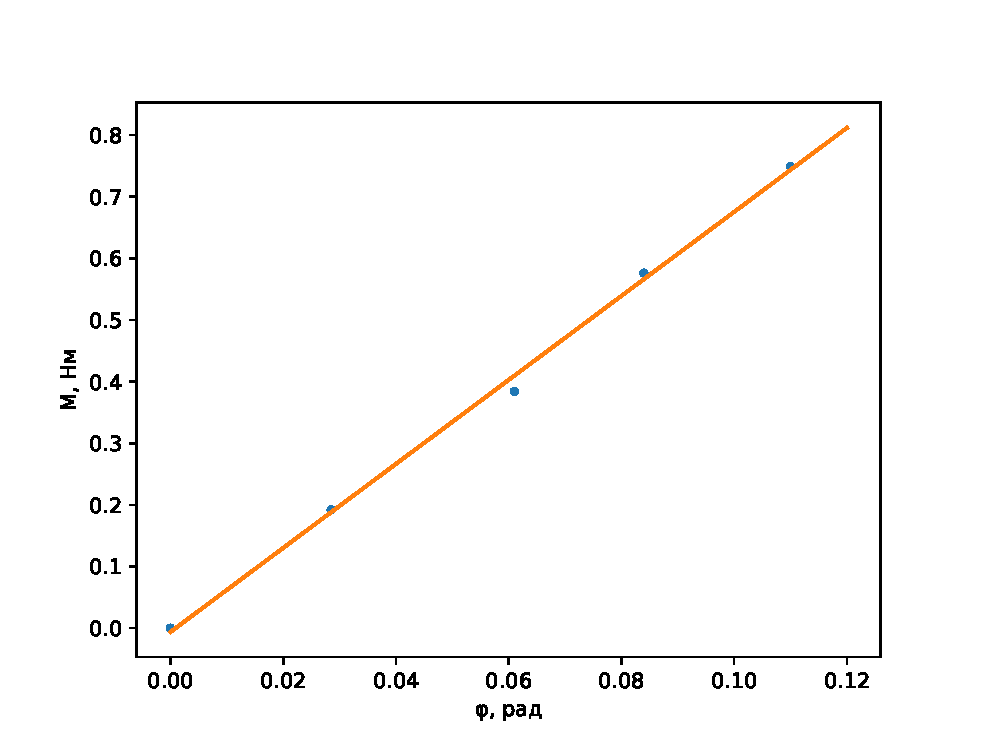
\includegraphics[scale = 0.7]{static.eps}

По МНК получаем:
\begin{align*}
f_0 &= 6.81 \text{Нм} \\
\sigma^2 &= \frac{1}{5}\sum_{i=1}^5 (f_0 - f_i)^2 = 0.0575 \text{Нм}^2 \\
\Rightarrow f &= 6.8 \pm 0.24 \text{Нм}
\end{align*}

Зная значение $f$, посчитаем модуль сдвига $G$, пользуясь формулой (\ref{eq:fG}) на странице (\pageref{eq:fG})

\[
G = \frac{f2l}{\pi R^4} = 0.58 \pm 0.02 \text{ГПа}
\]

\subsection{Динамический метод}

Измерим диаметр проволоки $d_0$ = 1.55мм, её длину $L$ = 1.34м и массу подвешиваемых грузов $m$ = 0.376кг.
Снимем зависимость квадрата периода колебаний $T$ от квадрата расстояния от проводоки до центра масс каждого груза $l$:

\newpage
\begin{center}
\title{Зависимость $T^2(l^2)$} \\
\begin{tabular}{|l|l|}
\hline
$T^2$, $c^2$ & $l^2$, $10^{-3}m^2$ \\ \hline
4,84   & 3,025  \\ \hline
5,76   & 4,225  \\ \hline
7,29   & 5,635  \\ \hline
9,00   & 7,225  \\ \hline
10,89  & 9,025  \\ \hline
\end{tabular}
\end{center}

По данным значениям построим график:

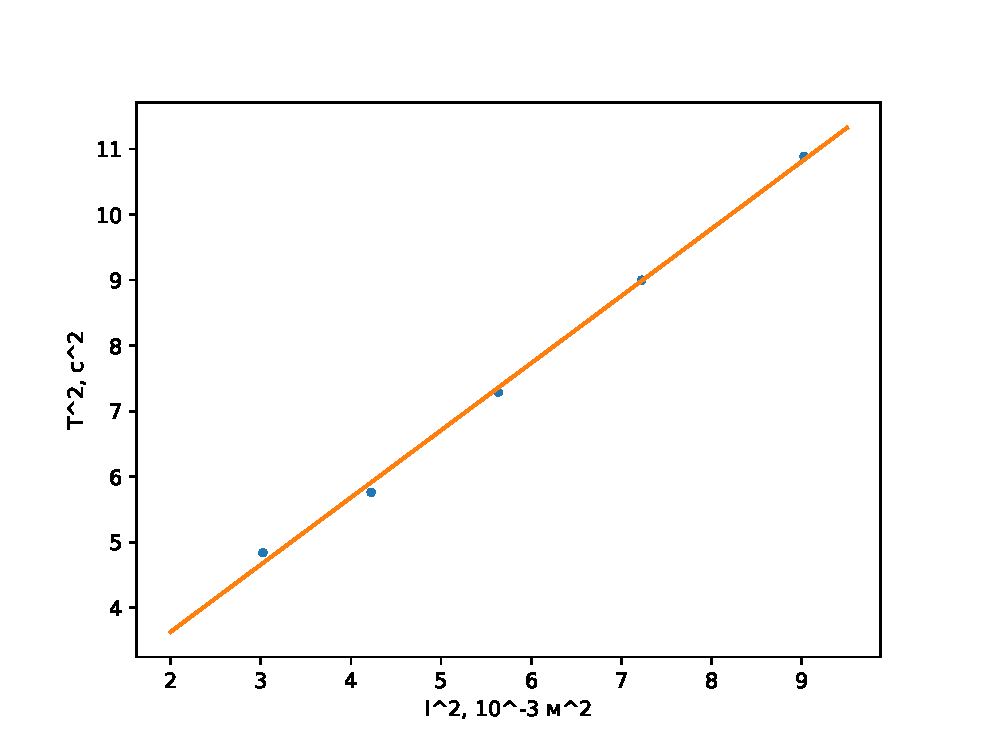
\includegraphics[scale = 0.7]{dynamic.eps}

По МНК найдем коэффициент наклона прямой:
\begin{align*}
k_0 &= 1,55 \frac{c^2}{10^{-3} \text{м}^2} \\
\sigma^2 &= \frac{1}{5}\sum_{i=1}^5 (k_0 - k_i)^2 = 0,065 \text{Нм}^2 \\
\Rightarrow k &= 1.55 \pm 0.25 \text{Нм}
\end{align*}

Из коэффициента $k$ найдем модуль кручения $f$ по формуле
\[
f = \frac{8\pi^2m}{k} = 19,67 \pm 3,18 \text{Нм}
\]

Зная значение $f$, посчитаем модуль сдвига $G$, пользуясь формулой (\ref{eq:fG}) на странице (\pageref{eq:fG})

\[
G = \frac{f2l}{\pi r^4} = 0.46 \pm 0.75 \text{ГПа}
\]

\section{Заключение}

Получив значения модуля кручения и модуля сдвига двумя различными способами и посчитав погрешность, мы можем увидеть,
что статический метод даёт более точный результат. Более точное значение достигается за счёт статичности установки.


\end{document}